\documentclass[11pt]{article}
\usepackage{../EllioStyle}
\usepackage{fancyvrb}
\usepackage{pdfpages}
\usepackage{xcolor}

\title{Homework 4}
\author{Elliott Pryor}
\date{15 Oct 2020}


\begin{document}
\maketitle


\problem{1}
\begin{figure}[H]
    \centering
    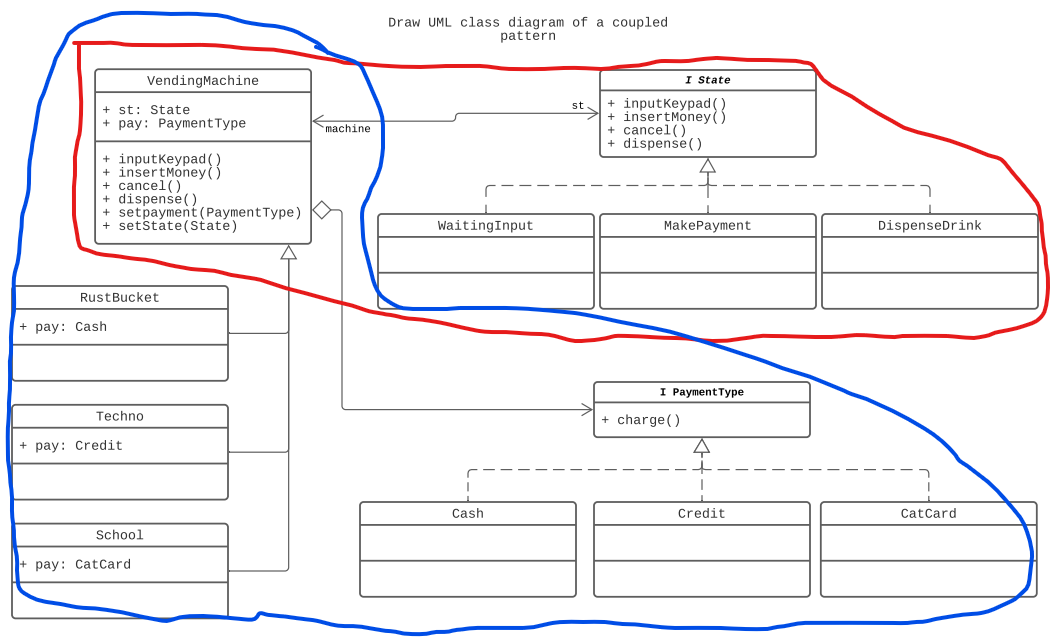
\includegraphics[scale=0.5]{./circled_components.png}
    \caption{Coupled components are circled}
    \label{fig:circled}
\end{figure}

In figure \ref{fig:circled}, the coupled components are circled. \textcolor{red}{The components circled in red are the state pattern}, and \textcolor{blue}{the components circled in blue are the strategy pattern}. This depicts a vending machine. There are multiple states the vending machine could be in (similar to the gumball machine from class). Each vending machine can use a different payment type (strategy pattern) that could be swapped out. So if money is inserted in the makePayment state it will use the pay object (type PaymentType) to collect money in a variety of ways. This combines the strategy pattern (changeable PaymentType) and the State pattern (different VendingMachine states).

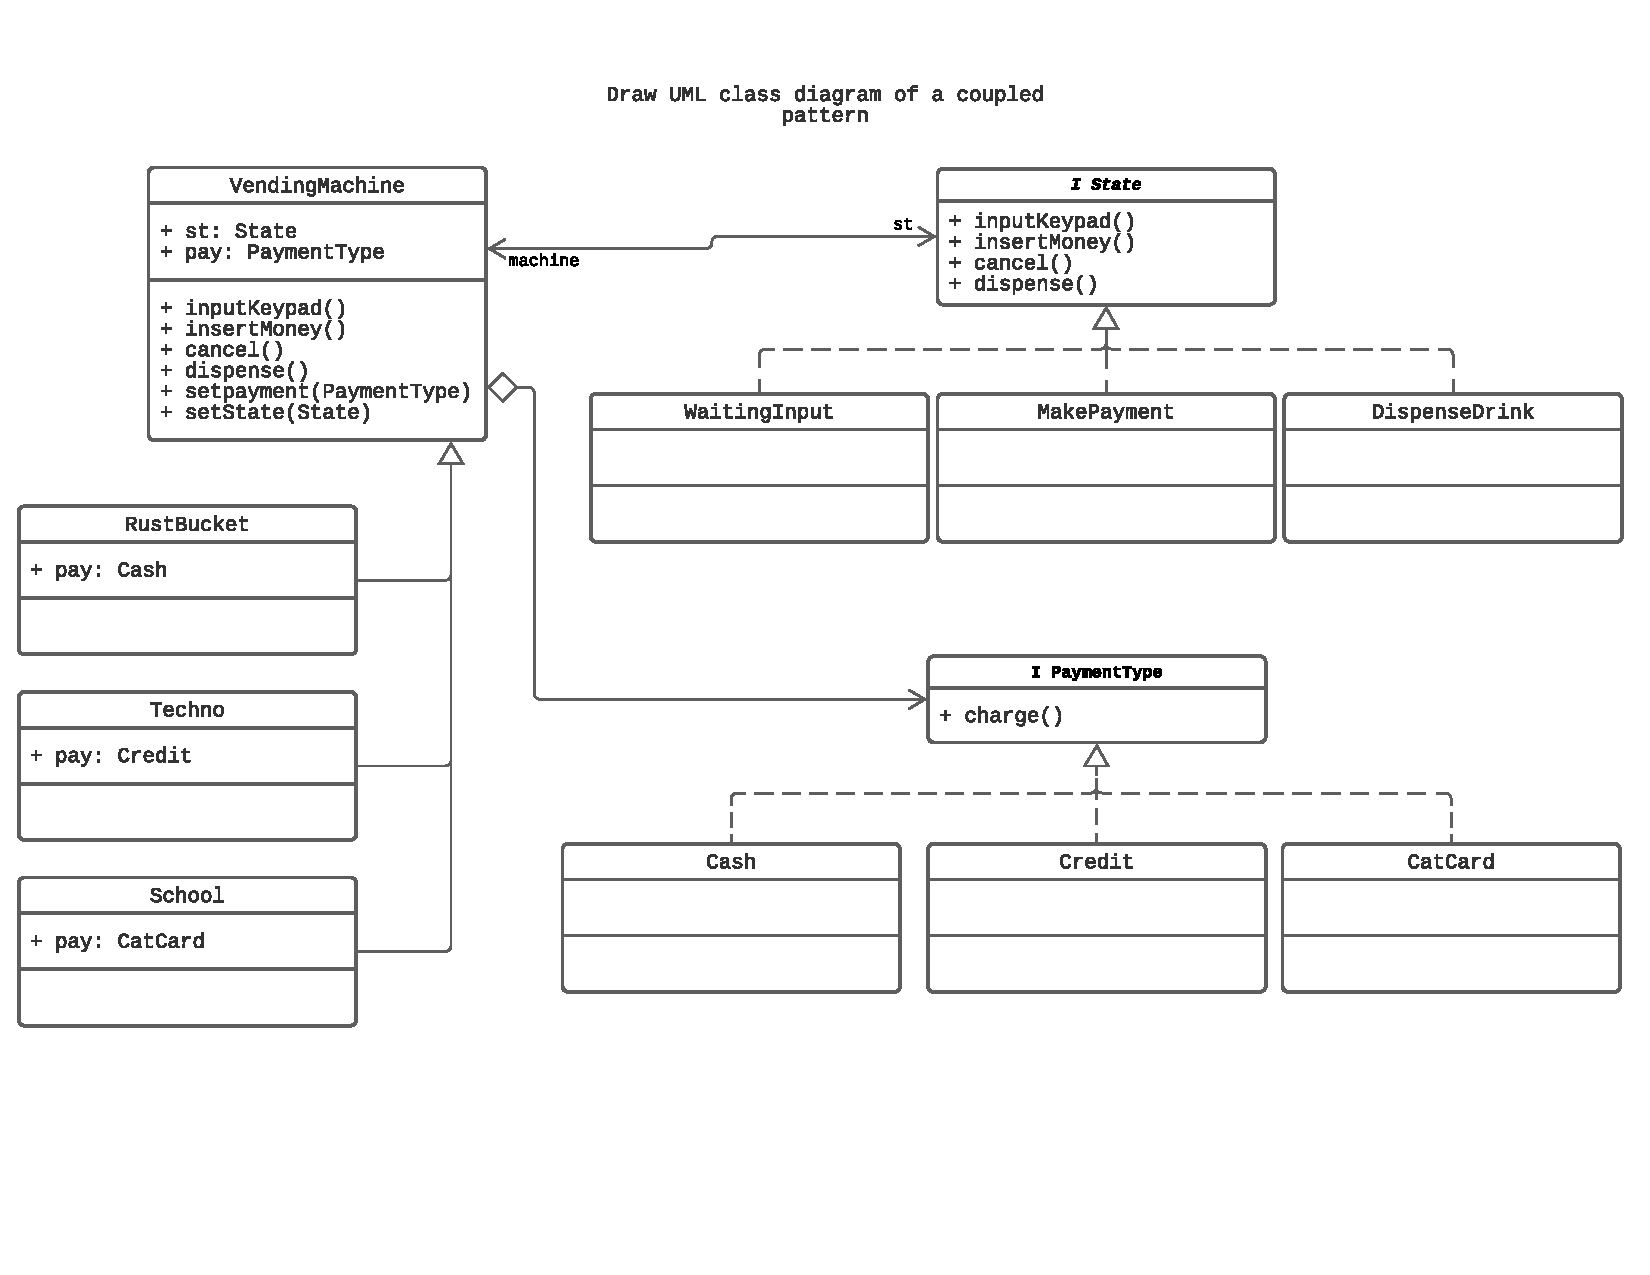
\includepdf[pages={1}]{./classDiagram.pdf}
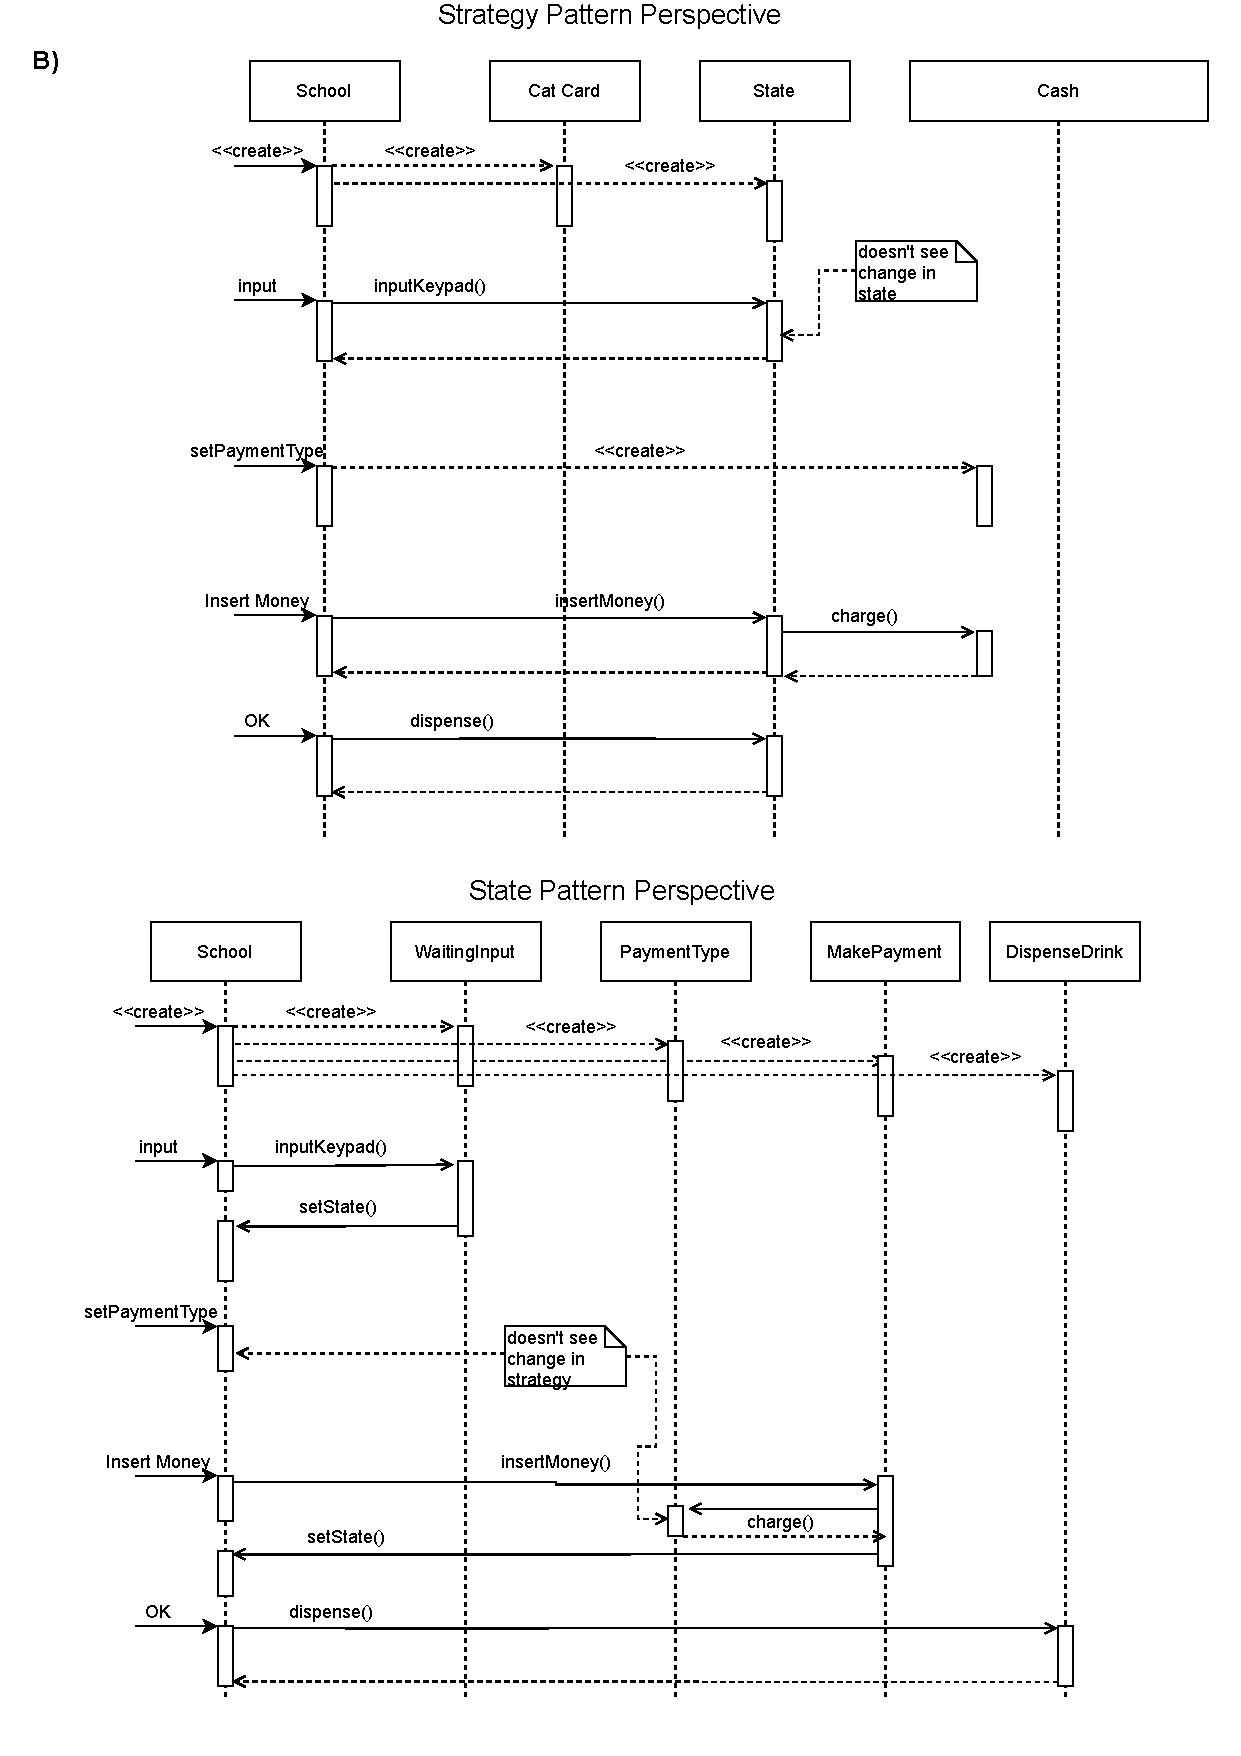
\includepdf[pages={1}]{./SequenceDiagram.pdf}


\problem{2}

\begin{enumerate}[a)]
\item What type of 'attack' was Mary Queen of Scots subject to?
\item How could Mary and Babington improved upon their solution?
\end{enumerate}

\hrule

\begin{enumerate}[a)]
\item Mary and Babbington were subject to a man in the middle attack. The courier intercepted the messages and pretended to be Mary. Babington and Mary had no way of verifying that the message actually came from. Their key was more-or-less cracked by a brute force method and frequency analysis. 

\item Practically, it would have been hard to avoid the issue, since the courier carried the key. Assuming that the cryptographer (Phelippes) did not have the key, then a key less prone to frequency analysis should be used. So having more characters in they key than 26 and having one key character represent sequences of english letters. Or use a Vigenere cipher which is a combination of shift ciphers and is more resistant to frequency analysis. Also a cipher that changes by the date would be more resistant to frequency analysis. 

Another solution would be to use multiple couriers so that one traitor cannot disrupt the entire communications. 
\end{enumerate}



 





\end{document}